%% FEUP THESIS STYLE for LaTeX2e
%% how to use feupteses (portuguese version)
%%
%% FEUP, JCL & JCF, 31 Jul 2012
%%
%% PLEASE send improvements to jlopes at fe.up.pt and to jcf at fe.up.pt
%%

%%========================================
%% Commands: pdflatex tese
%%           bibtex tese
%%           makeindex tese (only if creating an index) 
%%           pdflatex tese
%% Alternative:
%%          latexmk -pdf tese.tex
%%========================================

\documentclass[11pt,a4paper,twoside,openright]{report}

%% For iso-8859-1 (latin1), comment next line and uncomment the second line
\usepackage[utf8]{inputenc}
%\usepackage[latin1]{inputenc}

%% Portuguese version

%% MIEIC options
\usepackage[portugues,mieic]{feupteses}
%\usepackage[portugues,mieic,juri]{feupteses}
%\usepackage[portugues,mieic,final]{feupteses}
%\usepackage[portugues,mieic,final,onpaper]{feupteses}

%% Options: 
%% - portugues: titles, etc in portuguese
%% - onpaper: links are not shown (for paper versions)
%% - backrefs: include back references from bibliography to citation place

%% Uncomment the next lines if side by side graphics used
%\usepackage[lofdepth,lotdepth]{subfig}
%\usepackage{graphicx}
%\usepackage{float}

%% Include color package
\usepackage{color}
\definecolor{cloudwhite}{cmyk}{0,0,0,0.025}

%% Include source-code listings package
\usepackage{listings}
\lstset{ %
 language=C,                        % choose the language of the code
 basicstyle=\footnotesize\ttfamily,
 keywordstyle=\bfseries,
 numbers=left,                      % where to put the line-numbers
 numberstyle=\scriptsize\texttt,    % the size of the fonts that are used for the line-numbers
 stepnumber=1,                      % the step between two line-numbers. If it's 1 each line will be numbered
 numbersep=8pt,                     % how far the line-numbers are from the code
 frame=tb,
 float=htb,
 aboveskip=8mm,
 belowskip=4mm,
 backgroundcolor=\color{cloudwhite},
 showspaces=false,                  % show spaces adding particular underscores
 showstringspaces=false,            % underline spaces within strings
 showtabs=false,                    % show tabs within strings adding particular underscores
 tabsize=2,	                    % sets default tabsize to 2 spaces
 captionpos=b,                      % sets the caption-position to bottom
 breaklines=true,                   % sets automatic line breaking
 breakatwhitespace=false,           % sets if automatic breaks should only happen at whitespace
 escapeinside={\%*}{*)},            % if you want to add a comment within your code
 morekeywords={*,var,template,new}  % if you want to add more keywords to the set
}

%% Uncomment next line to set the depth of sectional units listed in the toc
%\setcounter{tocdepth}{3}

%% Uncomment to create an index (at the end of the document)
%\makeindex

%% Path to the figures directory
%% TIP: use folder ``figures'' to keep all your figures
\graphicspath{{figures/}}

%%----------------------------------------
%% TIP: if you want to define more macros, use an external file to keep them
%some macro definitions

% format
\newcommand{\class}[1]{{\normalfont\slshape #1\/}}

% entities
\newcommand{\Feup}{Faculdade de Engenharia da Universidade do Porto}

\newcommand{\svg}{\class{SVG}}
\newcommand{\scada}{\class{SCADA}}
\newcommand{\scadadms}{\class{SCADA/DMS}}

%%----------------------------------------

%%========================================
%% Start of document
%%========================================
\begin{document}

%%----------------------------------------
%% Information about the work
%%----------------------------------------
\title{Título da Dissertação}
\author{Nome do Autor}

%% Uncomment next line for date of submission
%\thesisdate{31 de Julho de 2008}

%% Uncomment next line for copyright text if used
%\copyrightnotice{Nome do Autor, 2008}

\supervisor{Orientador}{Nome do Orientador}

%% Uncomment next line if necessary
%\supervisor{Co-orientador}{Nome de Outro Orientador}

%% Uncomment committee stuff in the final version
%\committeetext{Aprovado em provas públicas pelo Júri:}
%\committeemember{Presidente}{Nome do presidente do júri}
%\committeemember{Arguente}{Nome do arguente do júri}
%\committeemember{Vogal}{Nome do vogal do júri}
%\signature

%% Specify cover logo (in folder ``figures'')
\logo{uporto-feup.pdf}

%% Uncomment next line for additional text below the author's name (front page)
\additionalfronttext{Preparação da Dissertação}

%%----------------------------------------
%% Preliminary materials
%%----------------------------------------

% remove unnecessary \include{} commands
\begin{Prolog}
  \chapter*{Resumo}

Assim como no desenvolvimento de software onde os bugs devem ser detectados e corrigidos o mais rapidamente possível, a validação de hardware está ao mesmo nível de prioridade quando usada em aplicações que procuram reduzir drasticamente os custos e estender a vida útil dos sistemas.

\sloppy
Nestes sistemas embutidos complexos, vários sistemas de interface, tais como os Field-Programmable Gate Arrays (FPGAs), são distribuídos em vários blocos de hardware.

A interação entre os vários sistemas envolve uma integração do firmware e o seu hardware.
Com a complexidade crescente desses sistemas, especialmente nessa interação, é imperativo reduzir o tempo do processo de validação funcional do hardware.

Para se alcançar isso, propomos implementar um ambiente de hardware de validação automática, permitindo testes sistemáticos e automáticos no hardware, assim como mostrar métricas de desempenho do hardware com uma combinação específica de cada elemento na placa do sistema, como a versão do Driver no CPU, a versão do Verilog configurada no FPGA, assim como a própria versão da placa.

Nesta tese, realizada na Synopsys Porto, será descrita a estrutura de um ambiente de validação de testes automáticos em integração contínua, e aplicá-lo no contexto de validação de hardware. 

Será também delineado o processo de criação um painel com as diferentes informações relacionadas aos sistemas em teste, com o objetivo de ajudar os stakeholders numa equipa de desenvolvimento a ter uma vista dos resultados do processo mais simplificada.

\vspace*{10mm}\noindent

\noindent\textbf{Palavras Chave}: \emph{Continuous Integration}, \emph{Hardware Validation}

\vspace*{5mm}\noindent

\noindent\textbf{Classificação}: 
\begin{itemize}
\item \emph{Software and its engineering $\rightarrow$ Software creation and management $\rightarrow$ Software verification and validation}; 
\item \emph{Hardware $\rightarrow$ Hardware validation}
\end{itemize} % the abstract
  \chapter*{Agradecimentos}
%\addcontentsline{toc}{chapter}{Agradecimentos}

Aliquam id dui. Nulla facilisi. Nullam ligula nunc, viverra a, iaculis
at, faucibus quis, sapien. Cum sociis natoque penatibus et magnis dis
parturient montes, nascetur ridiculus mus. Curabitur magna ligula,
ornare luctus, aliquam non, aliquet at, tortor. Donec iaculis nulla
sed eros. Sed felis. Nam lobortis libero. Pellentesque
odio. Suspendisse potenti. Morbi imperdiet rhoncus magna. Morbi
vestibulum interdum turpis. Pellentesque varius. Morbi nulla urna,
euismod in, molestie ac, placerat in, orci. 

Ut convallis. Suspendisse luctus pharetra sem. Sed sit amet mi in diam
luctus suscipit. Nulla facilisi. Integer commodo, turpis et semper
auctor, nisl ligula vestibulum erat, sed tempor lacus nibh at
turpis. Quisque vestibulum pulvinar justo. Class aptent taciti
sociosqu ad litora torquent per conubia nostra, per inceptos
himenaeos. Nam sed tellus vel tortor hendrerit pulvinar. Phasellus
eleifend, augue at mattis tincidunt, lorem lorem sodales arcu, id
volutpat risus est id neque. Phasellus egestas ante. Nam porttitor
justo sit amet urna. Suspendisse ligula nunc, mollis ac, elementum
non, venenatis ut, mauris. Mauris augue risus, tempus scelerisque,
rutrum quis, hendrerit at, nunc. Nulla posuere porta orci. Nulla dui. 

Fusce gravida placerat sem. Aenean ipsum diam, pharetra vitae, ornare
et, semper sit amet, nibh. Nam id tellus. Etiam ultrices. Praesent
gravida. Aliquam nec sapien. Morbi sagittis vulputate dolor. Donec
sapien lorem, laoreet egestas, pellentesque euismod, porta at,
sapien. Integer vitae lacus id dui convallis blandit. Mauris non
sem. Integer in velit eget lorem scelerisque vehicula. Etiam tincidunt
turpis ac nunc. Pellentesque a justo. Mauris faucibus quam id
eros. Cras pharetra. Fusce rutrum vulputate lorem. Cras pretium magna
in nisl. Integer ornare dui non pede. 

\vspace{10mm}
\flushleft{O Nome do Autor}
  % the acknowledgments
  \cleardoublepage
\thispagestyle{plain}

\vspace*{8cm}

%\begin{flushright}
%   \textsl{``Our main business is not to see what lies dimly at a distance,\\ %but to do what lies clearly at hand.''} \\
%\vspace*{1.5cm}
%           Thomas Carlyle
\begin{flushright}
   \textsl{``Do. Or do not.\\ There is no try.''} \\
\vspace*{1.5cm}
           Master Yoda
\end{flushright}
    % initial quotation if desired
  \cleardoublepage
  \pdfbookmark[0]{Conteúdo}{contents}
  \tableofcontents
  \cleardoublepage
  \pdfbookmark[0]{Lista de Figuras}{figures}
  \listoffigures
  \cleardoublepage
  \pdfbookmark[0]{Lista de Tabelas}{tables}
  \listoftables
  \chapter*{Abreviaturas e Símbolos}
%\addcontentsline{toc}{chapter}{Abbreviations}
\chaptermark{ABREVIATURAS E SÍMBOLOS}

\begin{flushleft}
\begin{tabular}{l p{0.8\linewidth}}
ADT      & Abstract Data Type\\
ANDF     & Architecture-Neutral Distribution Format\\
API      & Application Programming Interface\\
CAD      & Computer-Aided Design\\
CASE     & Computer-Aided Software Engineering\\
CORBA    & Common Object Request Broker Architecture\\
UNCOL    & UNiversal COmpiler-oriented Language\\
Loren    & Lorem ipsum dolor sit amet, consectetuer adipiscing
elit. Sed vehicula lorem commodo dui\\
WWW      & \emph{World Wide Web}
\end{tabular}
\end{flushleft}

  % the list of abbreviations used
\end{Prolog}

%%----------------------------------------
%% Body
%%----------------------------------------

\StartBody

%% TIP: use a separate file for each chapter
\chapter{Introduction} \label{chap:intro}

\section*{}

Hardware validation process is essential when the hardware is used on complex embedded integrated systems in applications that pretend to reduce drastically the system costs and expand its durability\cite{TroyScott}.

In embedded systems, various interfaces are distributed by multiple blocs of hardware. The interaction between these systems wraps an integration of the Firmware and its respective hardware. Examples of these systems are the Reset and Clock, energy management, security and other blocks\cite{Abarbanel}.

Although the growing complexity of the systems, namely the interaction between firmware and hardware, the process of functional hardware validation needs to be drastically reduced and become more effective due to the "time-to-market". This requirement is even more relevant on the mobile communication industry, making the validation process a major part of the project development cost\cite{Puri-Jobi2015}.

These criteria motivate the creation of an automatic hardware validation environment, with characteristics that permit conducting systematic and automatic tests, as well as providing verification indicators tracking and test quality\cite{ShixiaoYan2015}\cite{Gupta11titleantares}.
%TODO

In this document we describe the development of a solution to help development teams track their work progress in their Jenkins projects. It is expected to help the validation process both in Hardware and Software development by creating a certain level of abstraction, so it can be applied to both

This chapter presents an introduction to the document, by making an overview of the problem, explaining our motivation and the goals we pretend to achieve and the dissertation structure.

\section{Context} \label{sec:context}

This Dissertation was proposed by Synopsys Portugal, chosen as the MSc Dissertation in Informatics and Computing Engineering of the Faculty of Engineering of the University of Porto.
It emerged from the need to monitor and exhibit the status of current projects in development to stakeholders not accustomed to the used development tools. In this case, the Jenkins CI.
%TODO

In order to mitigate the complexity of the problem, new validation techniques will have to be investigated in which functional requirements are verified by stimulating the Hardware with configurations and specific test sequences.

SNPS Portugal Lda office is located at Maia (Tecmaia) and it is one of the offices of Synopsys Inc, the leading American company by sales in the Electronic Design Automation industry. 

The Synopsys IPK R\&D team, the one collaborating with this project, is the team responsible for the validation process of the developed IP designs~\cite{snps:ipInitiative}, following a specific set of requirements and specifications to be verified accordingly a series of compliance tests defined by the technologies consortia~\cite{snps:hdmiConsortium}~\cite{snps:pciConsortium}.

This team raised the need of having a more centralized and reliable source of information regarding the validation process  of their projects. These projects consist of developing and optimizing the firmware utilized in HDMI and PCI-express sockets. 

\section{Problem Statement}

The subjectivity of validation process in any kind of software development requires the use of some type of structure and categorization of data. This can help an easier access in troubleshooting flaws in the development.

The hypothesis is that with our solution, the productivity in development teams will increase by having this information displayed in a streamlined, precise and straightforward way.

In order to validate this, the system has to be implemented in a real project and feedback collected by the team to understand if the value added is noticeable.


\section{Motivation and Goals} \label{sec:goals}

The hardware validation process is directly related with verifying if the different clients configurations will be fulfilled. As such, the validation process can become a subjective process, since it involves assessing how the behavior of the hardware will operate in the most diverse applications and conditions. The process typically consists of activities which include system modeling, prototyping and evaluation by the user.

With this dissertation, we helped to build up a continuous integration environment for hardware validation by developing a Jenkins plugin in form of a dashboard in order to help Synopsys R\&D teams on the hardware prototyping process. 

To achieve this, the goals for the dissertation are:

%TODO performance indicators?
\begin{itemize}
\item Define an automatic test management structure for Hardware validation;
\item Define techniques to label and manage the Hardware validation test results;
\item Development of an web application to support the automatic test system;
\item Test the web application and validate its usefulness.
\end{itemize}

\section{Document Structure} \label{sec:struct}

In addition to the introduction, this dissertation report contains 5 other chapters. 
Chapter~\ref{chap:sota} describes the state of the art and present related work.
Chapter ~\ref{chap:research_problem} presents the system we want to base our study on and test.
Chapter ~\ref{ch:solution} describes the implementation of our application.
Results and evaluation are shown in chapter ~\ref{chap:evaluation}.
Finally, in chapter~\ref{ch:concl}, is presented the conclusions and future work suggestions.
 
\chapter{State of the Art} \label{chap:sota}

\section*{}

In this chapter is described the state of the art of related work and technologies. It is divided in three parts. Section~\ref{sec:ci} is explained the Continuous Integration process. In section~\ref{sec:ci_tools} is presented the different tools for continuous integration in software development for future contextualization in hardware validation. In section~\ref{sec:hw_val_arc} is presented one hardware validation architecture in which will be based our solution.

\section{Continuous Integration}\label{sec:ci}

Continuous Integration (CI), in Software Engineering, is the process of merging all the working copies of developers to a shared mainline several times a day.
It was first mentioned by Grady Booch in his 1994 book "Object-Oriented Analysis and Design with Applications"~\cite{GradyBooch}, although he did not advocate integrating several times a day. 

Extreme programming (XP) adopted this concept, when Kent Beck described XP~\cite{KentBeck} as an agile methodology designed for improving productivity, flexibility and teamwork in projects, and did advocate integrating more than once per day, not leaving "unintegrated" code for more than a couple of hours, thus presenting CI as one of its practices.

CI was set to resolve prevent integration problems, referred to "Integration Hell" in early characterizations of XP, where developers used to divide work in modules, that once completed, would be integrated to create the application as a whole. It was a costly process in terms of time and effort, arising a number of bugs in the process.

The idea behind CI is to reduce this issues by integrating early and often, so as to avoid the "integration hell".

\subsection{Process}

Continuous Integration is a cyclic process, as seen in the figure \ref{fig:ci_process}, divided in the following steps:

\begin{enumerate}
\item \textbf{Commit -} Developer modifies the code, tests it and commits to the repository;
\item \textbf{Build -} Code is fetched from the repository, integrated and built;
\item \textbf{Test -} Tests are performed on the build, followed by a report of the outcome;
\item \textbf{Report -} Developers are notified about the build and tests results\\
\end{enumerate}

  \begin{figure}[H]
  \centering
      \makebox[\textwidth][c]{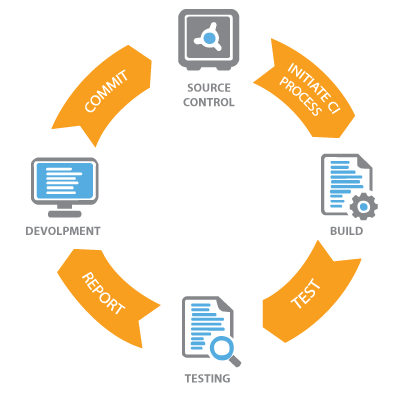
\includegraphics[width=0.5\textwidth]{ci_process}}
      \caption{Continuous Integration Process}
      \label{fig:ci_process}
  \end{figure}

The process is dependent of the build and tests duration. It is expected to be fast so it can be run several times a day.

\subsection{Components}\label{sc:ciComponents}
In this section are enumerated each component in the CI process.

\subsubsection{Developers}
Code developers are responsible for the creation of software. Continuous Integration is backed by several important principles and practices~\cite{CIimproveSQRR}:  

\begin{itemize}
\item \textbf{Check in frequently} - Frequent commits means that smaller amount of code changed, which leads to an easier process of finding bugs;
\item \textbf{Create automated tests} - Tests should be automated and have high code coverage;
\item \textbf{Don’t check in broken code} - Before commit, developers should test the code locally so errors aren't unnecessary introduced;  
\item \textbf{Don’t check in when the build is broken} - If a build is broken, it should be made top priority an effort in fixing it, so the errors do not propagate.
\end{itemize}

Many teams develop rituals around these policies, meaning the teams effectively manage themselves, knowing that if software is broken, they will receive immediate feedback.

\subsubsection{Repository}\label{repository}
A central repository with the project code using a Source Code Management (SCM) tool or Version Control System (VCS) is needed to perform a successful CI, maintaining the code reachable so the developers can get the most recent version of the source code.
This systems are important for software development as they serve as backup for programmers. It is possible to revert changes or pull previous code, allowing its use without the risk of breaking working code.
Repositories should contain the source code and everything else needed to create a build, such as: test files and scripts, database schemas, libraries and install scripts. Everything needed to run the software in a new machine.

\subsubsection{CI Server}
The CI server is the instrument behind Continuous Integration. It is used to implement continuous process of applying quality control of the software, by pulling the latest code from the repository, create a build and report the developers a feedback of the outcome.
There are several CI tools implementing this system, which we will talk in section \ref{sec:ci_tools} with more detail.

\subsection{Value}
By adopting Continuous Integration, you not only reduce risks and catch bugs quickly, but also move rapidly to working software.

With low-risk releases, you can quickly adapt to business requirements and user needs. This allows for greater collaboration between ops and delivery, fueling real change in your organization, and turning your release process into a business advantage.

\section{Continuous Integration Tools}\label{sec:ci_tools}

In order to set up a successful agile software development environment, it is essential to include a method of continuous integration in the process~\cite{Abdul2012}. This practice can be easily adapted to the hardware validation process, since it operates the same way as in software development:
\begin{enumerate}
\item Hardware logic is modified;
\item Firmware is built and deployed on the physical hardware;
\item Automated tests are run;
\item Hardware is validated.\\
\end{enumerate}

To contextualize this process into the hardware validation process, we must first choose a continuous integration tool before designing the architecture of the system.
It is known that there is a wide range of choices for continuous integration tools available, but for this project it was selected Jenkins as the preferred one. 

\subsection{Jenkins CI}\label{jenkins}

Jenkins~\cite{kn:Jenkins} is a continuous integration and continuous delivery tool application, used to build and test software projects and help developers integrate new changes and features to the project. It also provides ways to delineate customized build pipelines and integrate with several testing and deployment technologies.

It is the application of choice to create our system thanks to the several features it offers, such as:

\begin{itemize}
\item \textbf{Open Source} - Jenkins can be extended and modified in its majority, and makes uncomplicated to develop new plugins. This allows the creation of the dashboard plugin proposed;
\item \textbf{Automated Jobs / Jobs Management} - Jenkins can integrate with most software configuration management and build tools available. With this it is possible an easy script management of jobs to build, deploy and test the firmware developed;
\item \textbf{Build Reports} - The tool can automatically receive and generate logs of successful or failed builds, which can then be parsed (for example into an XML) and eventually used in a plugin or external application;
\item \textbf{Distributed System} - Jenkins can distribute builds and test loads to specific machines with the requested configurations.
\end{itemize}

\subsubsection{Jenkins Pipeline Jobs}\label{jenkinsPipeline}

In modern environment, delivering innovative ideas in a fast and reliable manner is extremely significant for any organization to better respond the dynamic market requirements \cite{Soni2015}. 

Recently, inside the Jenkins tool, was created a new ecosystem that allows implementing jobs in a domain specific language. It is referred to as Pipeline~\citet{jnks:pipeline} (formerly known as Workflow).

Pipeline is a powerful tool available for Jenkins users to implement various software delivery pipelines in code.

Since any peripheral hardware device can be attached to a Jenkins node, and these nodes requiring Java only, almost every development machine can be attached. A Sample scheme can be seen in the  figure~\ref{fig:connectionScheme}.

  \begin{figure}[H]
  \centering
      \makebox[\textwidth][c]{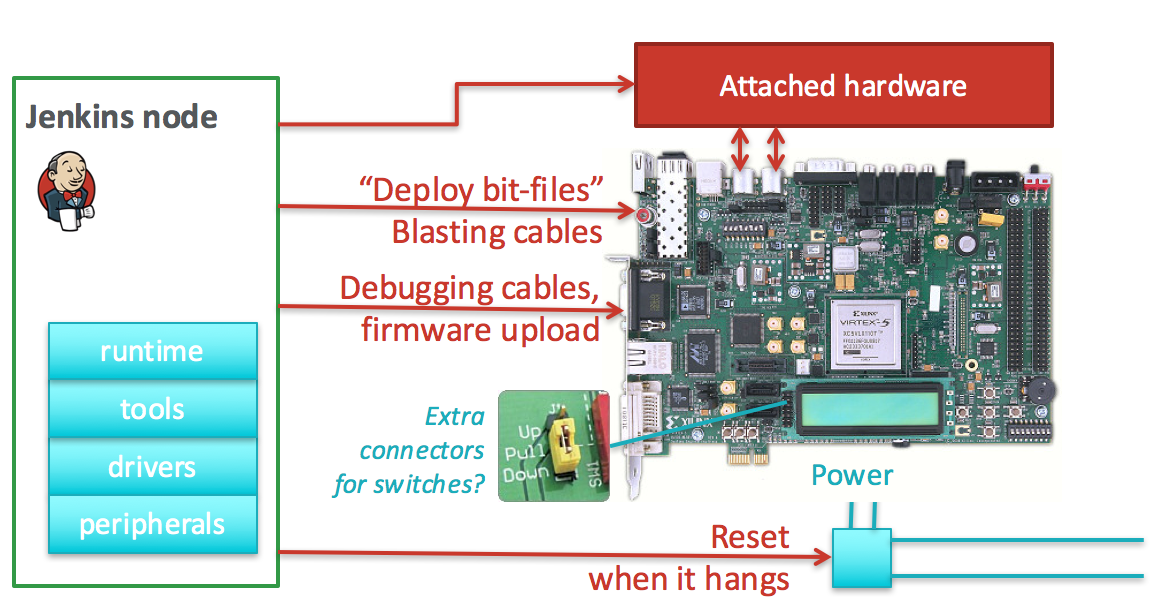
\includegraphics[width=1\textwidth]{connectBoard}}
      \caption{Common connection scheme ~\cite{jnks:automatedPipeline}}
      \label{fig:connectionScheme}
  \end{figure}
  
When connected, Jenkins jobs could invoke common EDA tools via command-line interfaces, which can be easily done by a Execute shell build steps in free-style projects.

Pipeline as Code is an approach for describing complex automation flows in software lifecycles, e.g: build, delivery, deployment.

In Jenkins there are two most popular plugins: Pipeline~\citet{jnks:pipeline} and Job DSL~\cite{jnks:dsl}. JobDSL Plugin internally generates common freestyle jobs according to the script, so it’s functionality is similar to the classic approaches. Pipeline is fundamentally different, because it provides a new engine controlling flows independently from particular nodes and workspaces. So it provides a higher job description level, which was not available in Jenkins before.

Accordingly to Oleg Nenashev~\cite{jnks:automatedPipeline}, there are several Pipeline features that may be of value to embedded and hardware projects.

\begin{itemize}
\item Robustness against restarts of Jenkins master.
\item Robustness against network disconnects. sh() steps are based on the Durable Task plugin~\cite{jnks:durableTask}, so Jenkins can safely continue the execution flow once the node reconnects to the master.
\item Possibility to run tasks on multiple nodes without creating complex flows based on job triggers and copy artifact steps. Achieved via combination of parallel() and node() steps.
\item Ability to store the shared logic in standalone Pipeline libraries
\end{itemize}

In conclusion, Jenkins is a powerful automation framework that can be used in many areas. Although it has no dedicated plugins for test runs on hardware, it provides diverse general-purpose "building blocks", that allow the implementation of any flow.

Pipeline as code can greatly simplify these complex implementations in Jenkins. It continues to evolve and extend support of use-cases.

\section{Hardware Validation Architectures}\label{sec:hw_val_arc}

Subsequently to deciding the CI tool to use, we must start designing the architecture of the target environment. The framework we came across that accomplishes our goal to some extent was the LAVA project.

\subsection{LAVA}\label{lava}

The Linaro Automated Validation Architecture (LAVA) project~\cite{kn:LAVA} is a "continuous integration system for deploying operating systems onto physical and virtual hardware for running tests". It can run simple boot loading and system level tests, where the results can be exported and inspected subsequently.

It is composed by two main components, as seen in the figure~\ref{fig:lava}: 

\begin{itemize}
\item The LAVA Server: a web application that provides a central scheduler, dashboard for job monitoring and test result visualization;
\item The LAVA Dispatcher: a sub-system that manages communication to the physical test devices.
\end{itemize}

The overall idea is allowing us to make continuous testing, quality control and automatic validation for projects of all sizes.

%Careful with this
\clearpage

\begin{figure}[H]
\centering
\makebox[\textwidth][c]{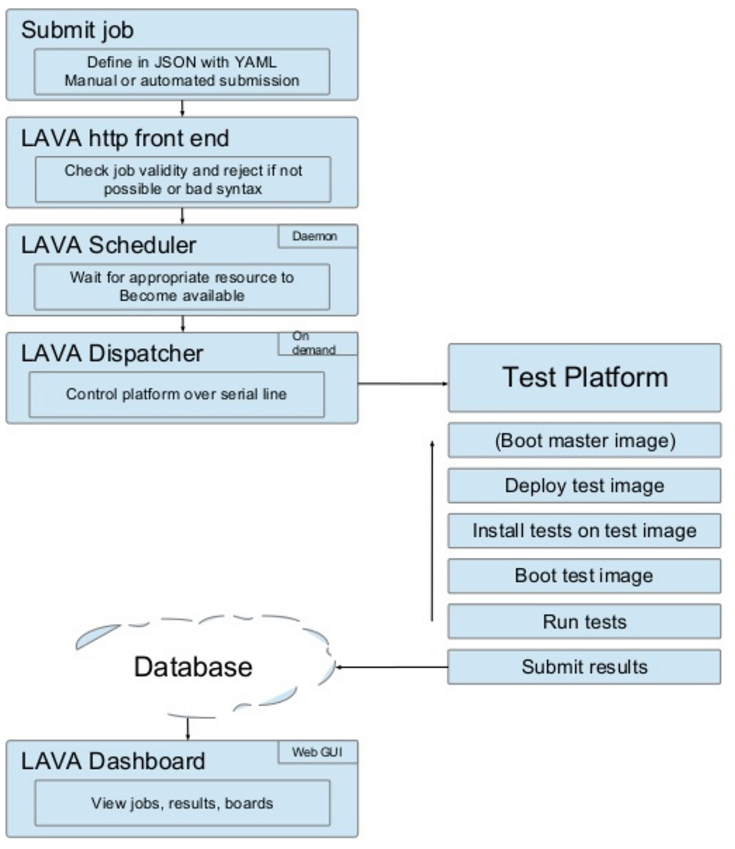
\includegraphics[width=1\textwidth]{lava_workflow}}
\caption{LAVA Workflow}
\label{fig:lava}
\end{figure}

It is to note that LAVA itself doesn't run the tests, it is only an enabler as it does not define what can be run. It is a merely black-box to CI, since the test jobs still have to be provided by an external source (usually Jenkins).\\
The framework serves to test the boards from the Linaro validation lab in Cambridge, where all devices have the same LAVA interface.

%https://www.youtube.com/watch?v=hS382L6EYrE
%http://www.slideshare.net/linaroorg/01-lava-introductionandupdatesdavemilo1

\section{Conclusions}
The market is full of CI tools available to use, but it is not very explored in the hardware validation context.

Since Synopsys already started to implement a Continuous Integration environment using Jenkins, with automated jobs by this time created in the application, and it providing key features for the goal system, makes sense to continue this approach to develop a new plugin for the tool.

Concluding, we can adapt the LAVA architecture to Synopsys interfaces using Jenkins, by using the job management and distributed system features as the central scheduler and dispatcher, and creating the dashboard plugin to supervise the test results.

\chapter{Research Problem} \label{chap:research_problem}

In this chapter, we present how the Continuous Integration System of the R\&D IPK team in Synopsys Porto is arranged and what needs to be improved. 

We will describe its architecture in section~\ref{sec:res_system}, with a little description of its different communication interfaces in section~\ref{sec:interfaces} and current continuous integration flow in section~\ref{sc:workflow}. It is also listed the requirements we will implement in the solution in section~\ref{sc:requirements}, following by the current method of displaying the project builds information in section~\ref{sec:spreadsheet}.
Finally a conclusion in section~\ref{sec:conclusion_3} about the problem in study.

\section{The System architecture}\label{sec:res_system}

Most compliance tests take long periods to finish (aprox. 4 hours, as displayed in the figure~\ref{fig:buildView} top-right corner). In addition to setting up and recreating the test environment for each run, it is felt as a waste of time. The current test automation environment, due to its manual labor has some issues such as the inconsistency between tests and the lack of traceability among product versions in testing. Hereupon, we want to increase efficiency and productivity of the R\&D teams in HW/SW testing and improve reporting to these teams.

To this goal, it is desirable to create an automated test architecture that eliminates the need of employing an engineer to configure the equipment by using automated test equipment, which will allow the continuous testing of different features configurations through automation. By consequence this permits an improved and robust test coverage, as well as increasing their number and velocity. This will summarize in a more refined and consistent testing process, with an improved degree of trust and certainty on the results.

This architecture should meet the following requirements:

\begin{itemize}
\item Speed up testing to allow for accelerated releases which:
	\begin{itemize}
		\item Reduces testing costs;
        \item Reduces time in testing phase.
	\end{itemize}
\item Allow testing IP's features continuously;
\item Improve test coverage;
\item Ensure consistency;
\item Improve the reliability of testing;
	\begin{itemize}
		\item Consolidate the testing process
	\end{itemize}
\end{itemize}

  \begin{figure}[H]
  \centering
      \makebox[\textwidth][c]{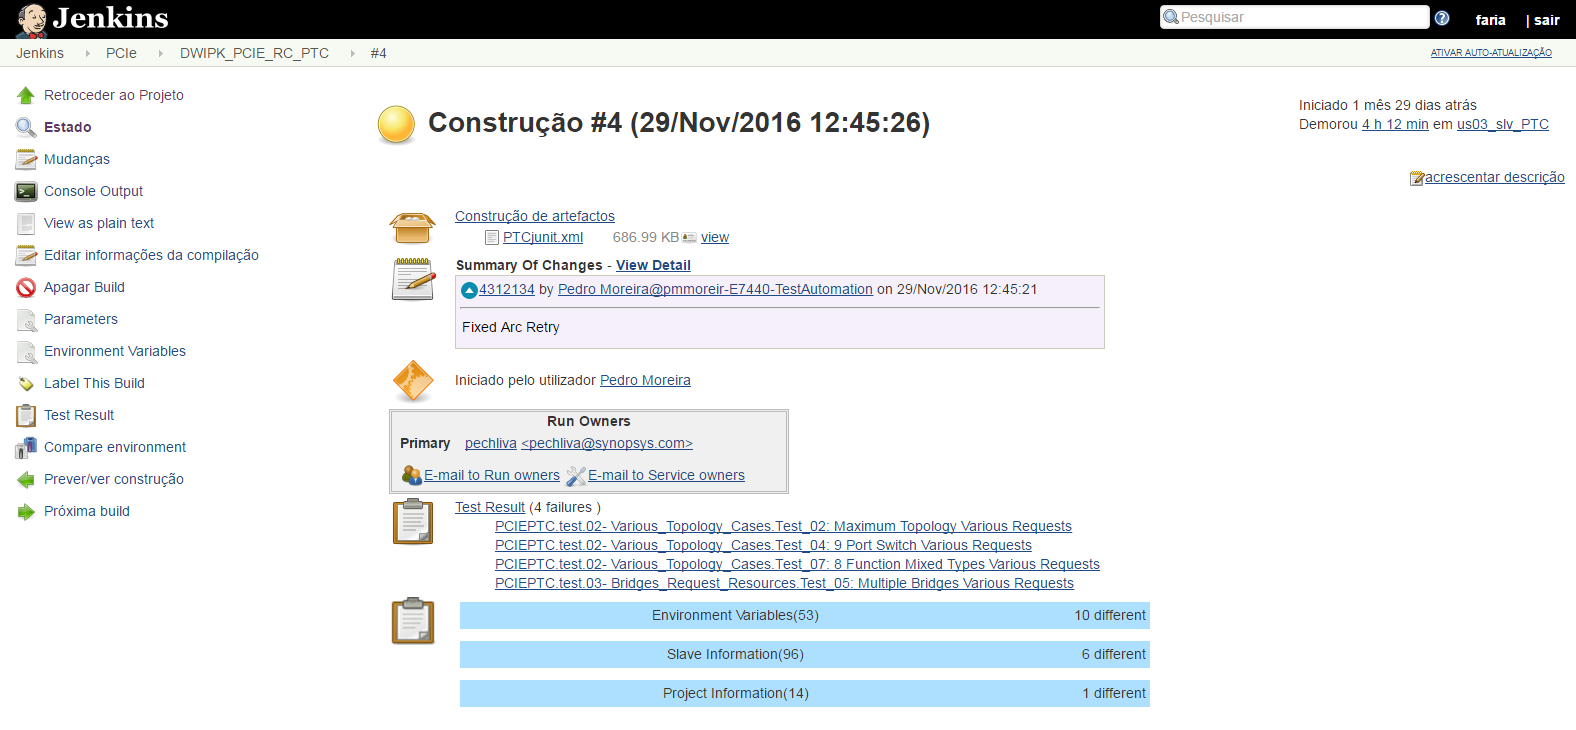
\includegraphics[width=1\textwidth]{buildViewInfo}}
      \caption{View of an example Build}
      \label{fig:buildView}
  \end{figure}

The block diagram shown in the figure~\ref{fig:ci_hw_context} shows the hardware testing architecture which is analogous to a common continuous integration software development setup.

\clearpage

  \begin{figure}[H]
  \centering
      \makebox[\textwidth][c]{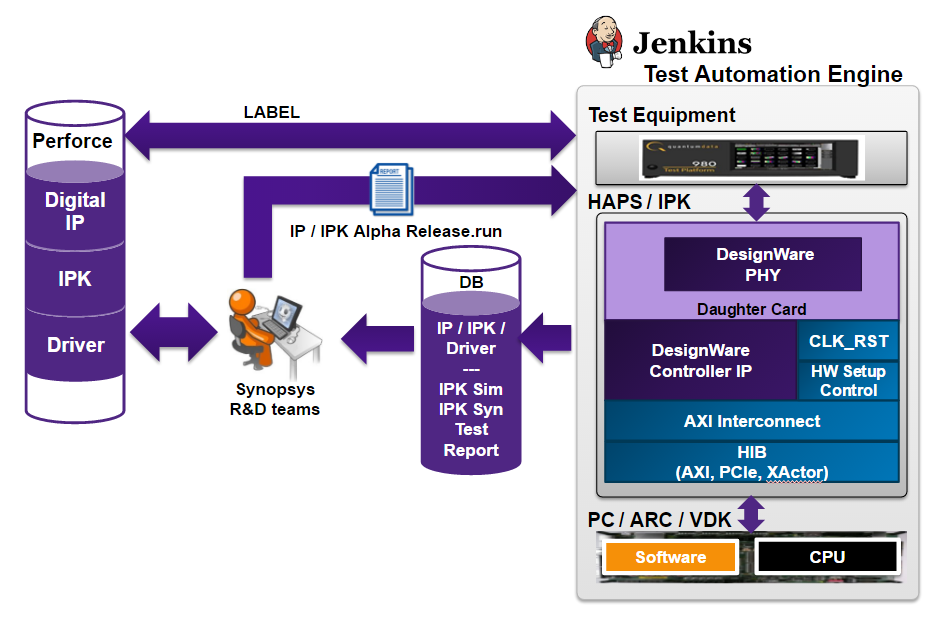
\includegraphics[width=1\textwidth]{ci_system_arch}}
      \caption{CI environment for Hardware Validation Context}
      \label{fig:ci_hw_context}
  \end{figure}
  
  
This architecture contains all the components used for a successful CI environment, as described in section \ref{sc:ciComponents}, being the object of test and analysis the multiple IP configurations, for the different communication interfaces, namely PCIe and ARC (see sections \ref{sc:pcie} and \ref{sc:arc}).

\subsection{Communication Interfaces}\label{sec:interfaces}

Here are succinctly described the HAPS platform and the different communication interfaces utilized as test objects by the IPK team. 

\subsubsection{HAPS}\label{sc:haps}

HAPS (High-performance ASIC Prototyping Systems) is an integrated and scalable hardware-software solution utilized by design and verification teams to improve their ASIC design schedules and avoid costly device re-spins\cite{HAPS}.

This prototyping solution consists of a collection of modular, easy-to-use products for ASIC and SoC prototyping that include HAPS hardware components supported by an integrated software tool flow for design planning, FPGA synthesis, and debug.

  \begin{figure}[H]
  \centering
      \makebox[\textwidth][c]{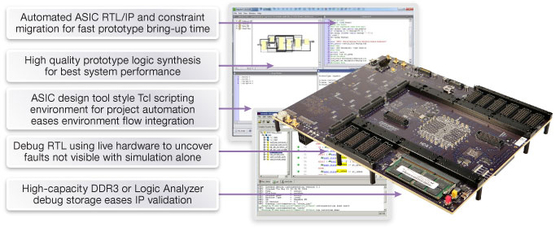
\includegraphics[width=0.5\textwidth]{haps}}
      \caption{HAPS®-Developer eXpress (HAPS-DX)}
      \label{fig:haps}
  \end{figure}

\subsubsection{ARC}\label{sc:arc}

Synopsys' DesignWare® ARC® Processors\cite{sns:ARC} are a family of 32-bit CPUs that SoC designers can optimize for a wide range of uses, from deeply embedded to high-performance host applications in a variety of market segments, such as Automotive and Industrial, Internet of Things or mobile. 

Designers can adapt their products by using configuration technology to tailor each ARC processor instance to meet specific performance, power and area requirements. These processors are also extendable, allowing designers to add their own custom instructions to increase performance.

  \begin{figure}[H]
  \centering
     \makebox[\textwidth][c]{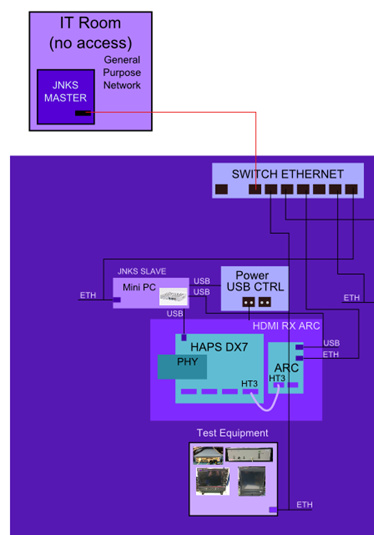
\includegraphics[width=0.5\textwidth]{arc}}
      \caption{ARC interface architecture}
     \label{fig:arc}
  \end{figure}


\subsubsection{PCIe}\label{sc:pcie}

PCI Express (Peripheral Component Interconnect Express), is a high-speed serial computer expansion bus standard, designed to replace the older bus standards\cite{wik:PCIE}\cite{sns:PCIE}.  Recent revisions of the PCIe standard provide hardware support for I/O virtualization.

The PCI Express electrical interface is also used in a variety of other standards, most notably in ExpressCard as a laptop expansion card interface, and in SATA Express as a computer storage interface.


 \begin{figure}[H]
  \centering
      \makebox[\textwidth][c]{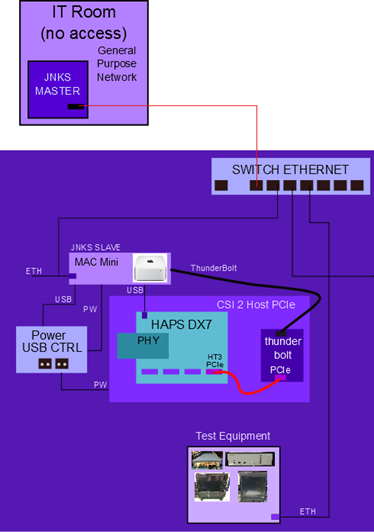
\includegraphics[width=0.5\textwidth]{pcie}}
      \caption{PCI Express (PCIe) interface architecture}
      \label{fig:pcie}
 \end{figure}

\subsection{CI-flow}\label{sc:workflow}

To better understand how the test automation for hardware/software validation works, the rundown of the process is described as follows:

\renewcommand{\labelenumii}{\theenumii}
\renewcommand{\theenumii}{\theenumi.\arabic{enumii}.}

\begin{enumerate}

\item The R\&D teams create an hardware image with a specific IP configuration to be deployed to the HAPS platform. At the same time, a firmware is packaged with its specific drivers to be deployed in the target interface, e.g. ARC and PCIe;

\item These files are committed to a VCS repository;

\item The Jenkins Master node receives notification of these changes and proceeds to run the associated Job. The Job is dispatched to the appropriate slave node, as seen in the figures \ref{fig:pcie} and \ref{fig:arc}, in a test automation rack that will trigger a set of sub-steps:

\begin{enumerate}
\item program the HAPS FPGA with the submitted hardware image;
\item boot the host interface and loads the firmware;
\item run a set of tests (IP compliance tests) from the test equipment and a log is generated;
\end{enumerate}

\item\label{failStep} The log is then parsed and a spreadsheet (detailed in section \ref{sec:spreadsheet}), containing all the relevant information is created. The spreadsheet is then validated by the R\&D teams.

\end{enumerate}

The last step of this flow is is faulted mainly by three dissatisfactory characteristics:

\begin{itemize}

\item The use of a spreadsheet file, which we detail its faults thoroughly in section~\ref{sec:spreadsheet}, that has no correlation with the Jenkins environment;

\item Jenkins default views of the IP projects do not display enough information to reach conclusions about the test results with ease;

\item Jenkins build views do not contain specific information about the configuration of the tested hardware, as seen in the figure \ref{fig:buildView}.

\end{itemize}

Ultimately, these are the points we want to correct in order to improve the last step, with this dissertation work.

\section{Solution Requirements}\label{sc:requirements}

For the display of the desired information in order for a better test result analysis, it was decided to implement a dashboard plugin as solution. Since dashboards allow stakeholders to monitor the contribution of the various elements in the organization. They allow the display of specific data points of the system in question, provided in a single "snapshot" \cite{dashboard}.

Presently, R\&D teams utilize an Excel spreadsheet created by its IP Prototyping Team, where most of the time the data is manually input with the test results obtained from a test compliance log. This method is a poor solution since it does not provide consistency between tests, nor automatic traceability among the different tested versions, as explained in section \ref{sec:spreadsheet}.

The dashboard plugin will serve as a project monitoring view where the R\&D teams can constantly observe the results of the hardware validation phase testing. The main features of the dashboard include:

\begin{itemize}
\item View customized to each development team;
\item Information of each test configuration;
\item Display of test results and build performance indicators (e.g. build average time of each configuration).
%\item Possibility of executing new tests with available alternative configurations.
\end{itemize}

\subsection{Project Views Alignment}\label{sc:projOrg}

The R\&D Jenkins environment is currently organized by different Views, each referencing a different project. As seen in the figure~\ref{fig:allViews}, a project View is very unidimensional, not displaying enough information.

Aware that each R\&D team can have more than one Project associated to it, this is one requirement we had in mind while creating our solution, as explained in section \ref{sc:implementationDesign}.

  \begin{figure}[H]
  \centering
      \makebox[\textwidth][c]{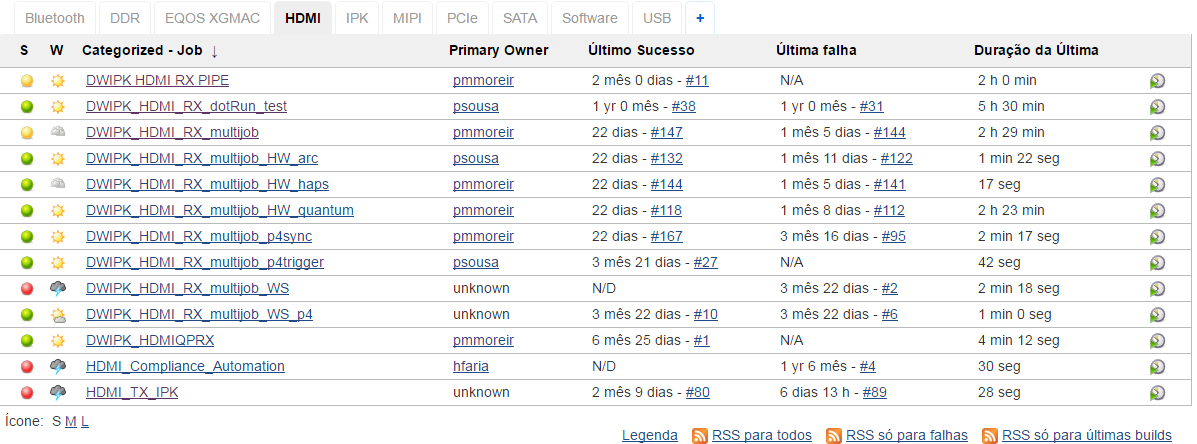
\includegraphics[width=1\textwidth]{allViews}}
      \caption{Project Views organized in the Jenkins system.}
      \label{fig:allViews}
  \end{figure}

\section{Project Build Spreadsheet}\label{sec:spreadsheet}

The IPK team uses an Excel Spreadsheet to track the overall status of each job with different test configurations, illustrated in figures \ref{fig:excel1} and \ref{fig:excel2}. 

  \begin{figure}[H]
  \centering
      \makebox[\textwidth][c]{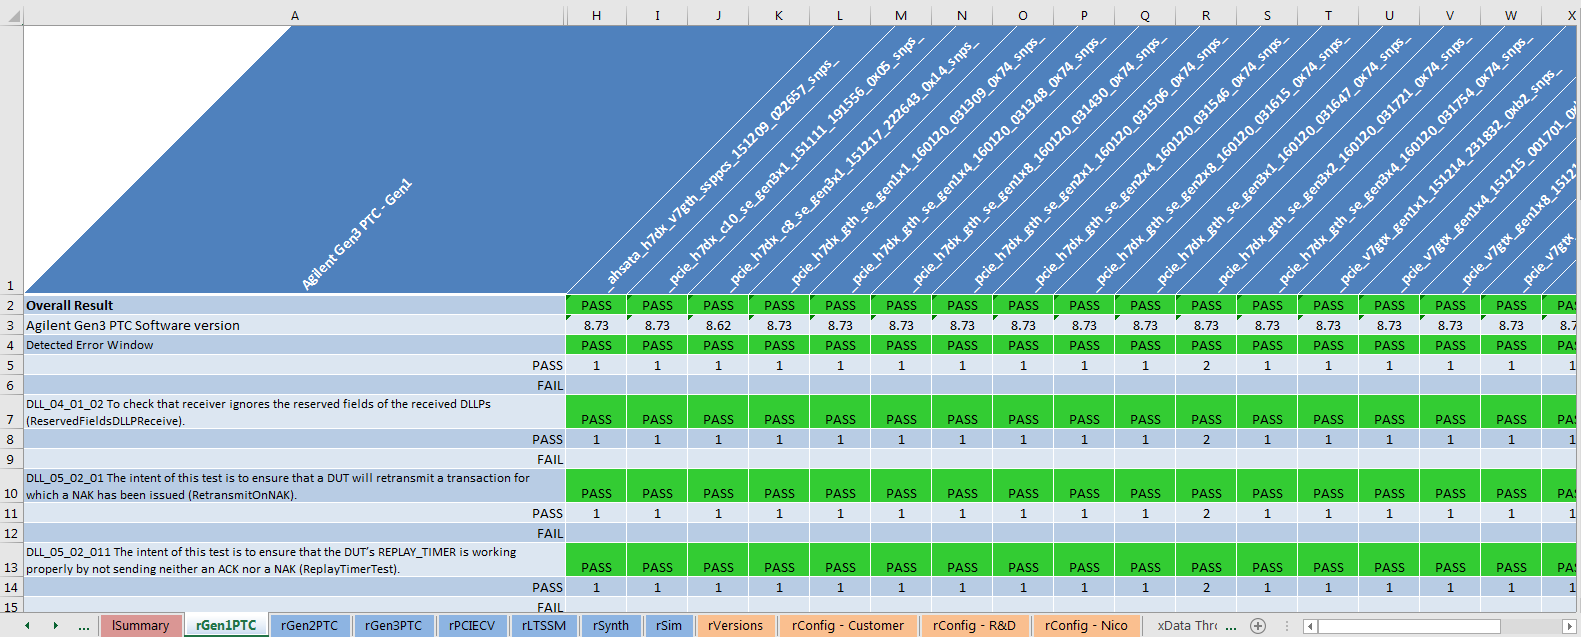
\includegraphics[width=1\textwidth]{excel1}}
      \caption{Hardware Test Summary Results}
      \label{fig:excel1}
  \end{figure}
  
Figure \ref{fig:excel1} depicts an example build run information in a PCIe interface. It is structured by the following elements:

\begin{itemize}
\item The labels in line 1 contain the project information, about the hardware build, namely the host interface, the PHY\cite{PHY} and top level hardware configurations, and date of the build;

\item The subsequent rows contain the test details, with the columns displaying information about the test result.
\end{itemize}
  
    \begin{figure}[H]
  \centering
      \makebox[\textwidth][c]{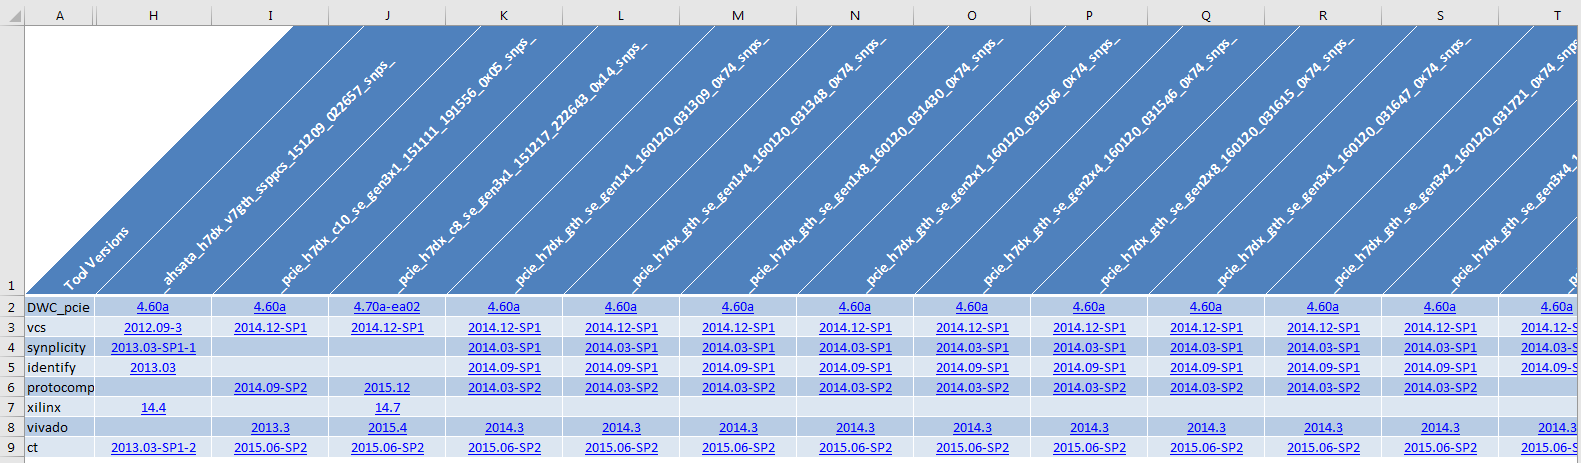
\includegraphics[width=1\textwidth]{excel2}}
      \caption{Different tools and controller Versions}
      \label{fig:excel2}
  \end{figure}

In figure \ref{fig:excel2} it is represented more information about the same build run, in a different sheet, showing the Controller Version in the first line, followed with the used tool versions for each configuration.

This exposes various problems, such as:

\begin{itemize}
\item \textbf{Traceability - } A new spreadsheet has to be created each time a new data-set of test results is created.
\item \textbf{Susceptible to Human Error - } If an error while populating the spreadsheet data is encountered, a manual fix is needed to correct it.
\item \textbf{Availability - } Every stakeholder in the process needs a copy of the spreadsheet for analysis.
\item \textbf{Difficulty to troubleshoot - } The need of correcting a failed test leads the user to search for it in the system.
\end{itemize}

A dashboard inside Jenkins will resolve this issues by aggregating the information in a single snapshot.

\section{Conclusion}\label{sec:conclusion_3}

Accuracy and speed need to be improved in the hardware validation process. Having a more centralized information access would greatly aid this improvement. 

Despite the fact that the organization of each project is well structured in Views, there is the need of a factor that facilitates its analysis, eliminating some of irrelevant information displayed.

The current solution is inefficient, with information disperse and more than required for the time being.

With this, it is safe to assume a View in form of a dashboard inside Jenkins is one optimal way to achieve this goal. Jenkins has a great API that allows access of its items inside its various Extension Points~\cite{jnks:extensionpoints}.

This will eliminate the issues of using a spreadsheet, since all the information is retrieved automatically from the Jenkins server in a reliable manner, and displayed available to every user inside the tool. It will make the validation process faster, concentrating the relevant information in a single view.
\include{chapter4}
\chapter{The Dashboard Solution}\label{ch:solution}

\section*{}

In this chapter, we will describe the Dashboard solution, its implementation and methodology under its development.

Since Synopsys had already setup the CI server in Jenkins, it was chosen to develop the Plugin for it. We also take the avantage of Jenkins being very customizable, with hundreds of extension points and plugins available to support our needs~\cite{kn:Jenkins}~\cite{jnks:extensionpoints}.

Nonetheless, it is not a simple task to develop a plugin due to lack of documentation. In order to find out how plugins work, it was crucial to look into other plugins source code.

Our plugin, named \textbf{Filtered Dashboard View} plugin~\cite{jksn:myplugin}, will be referenced from here on simply as \textbf{Dashboard}.

\section{Use Cases}\label{sc:usecases}

Taking into consideration the R\&D project organization of Jenkins, described in section \ref{sc:projOrg}, it was discussed with the collaborating IPK team that the best option was to develop the Dashboard as a View plugin, implementing the class ViewGroup, in order to aggregate different views inside it.

In the Use Case diagram in the figure ~\ref{fig:usecases} are pictured the actions a user can perform to display our Dashboard in the Jenkins environment. 

\newcommand{\code}{\texttt}



\begin{figure}
  \centering
      \makebox[\textwidth][c]{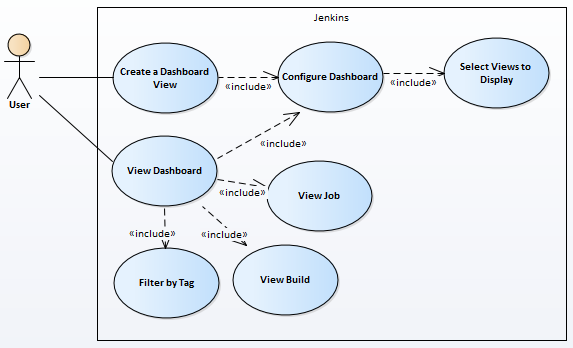
\includegraphics[width=1\textwidth]{usecases}}
      \caption{Dashboard plugin Use Case diagram}
      \label{fig:usecases}
\end{figure}  

The plugin is designed to be as simple as creating a new View inside the tool, selecting which other Views are requested to display, as shown in the figure \ref{fig:createView}. Afterwards, the user can freely change its configuration, namely add, remove or change which views will be displayed, demonstrated in the figure~\ref{fig:customize}.

It is important to note that all kinds of Views should be allowed to display inside the Dashboard, with the exception of itself and other instances of the same View Class, so no loops are originated from this process. 


    \begin{figure}[H]
        \begin{minipage}[b]{0.45\linewidth}
            \centering
            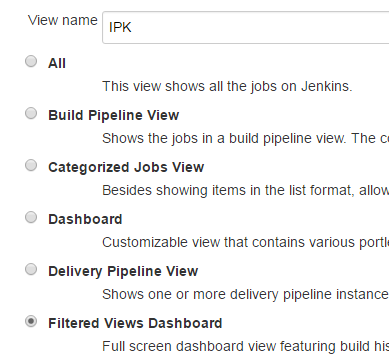
\includegraphics[width=\textwidth]{newview}
            \caption{View creation menu}
            \label{fig:createView}
        \end{minipage}
        \hspace{0.5cm}
        \begin{minipage}[b]{0.45\linewidth}
            \centering
            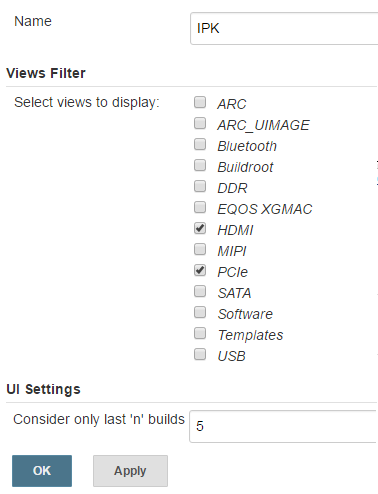
\includegraphics[width=\textwidth]{customiseview}
            \caption{Dashboard customization menu}
            \label{fig:customize}
        \end{minipage}
    \end{figure}

\section{Jenkins Plugin - Filtered Dashboard View}\label{sc:dashboard}

In this section it will be described the thought process of designing our plugin, including the research of similar and auxiliary plugins in \ref{sc:aux}, our implementation design in section~\ref{sc:implementationDesign}, and finally the display of the User Interface of the final product in section~\ref{sc:ui}.


\subsection{Auxiliary Plugins}\label{sc:aux}

Since Jenkins~\citet{kn:Jenkins} supports plugins, with an abundance of extension points which allow it to be extended to meet specific needs of individual projects, it was appropriate to investigate what similar plugins already exist that can be extended or modified as base to our own solution.

In this section, it will be described 2 plugins used to help achieve our final application.

\subsubsection{Mission Control Plugin}\label{mission_plugin}

Accounting that we want to create a Dashboard, we came across the Mission Control Plugin~\cite{jkns:missionC}, that has practically all the base to work with, a full dashboard view that features:

\begin{itemize}
\item Job status display;
\item Build history and build queue;
\item Extends a View Object~\cite{jnks:ViewObj}, which can be added to the main dashboard.
\end{itemize}

Despite being a starting point, the information displayed in the figure \ref{fig:missionControl}, needed to be trimmed and adapted to our requirements. 

Nevertheless, after making a profound source code analysis of this plugin, we had a good understanding on how we could interact with the Jenkins API in various ways, such as retrieving information of all necessary items in our Jenkins instance, exportation of this information and its interaction with the front-end.

  \begin{figure}[H]
  \centering
      \makebox[\textwidth][c]{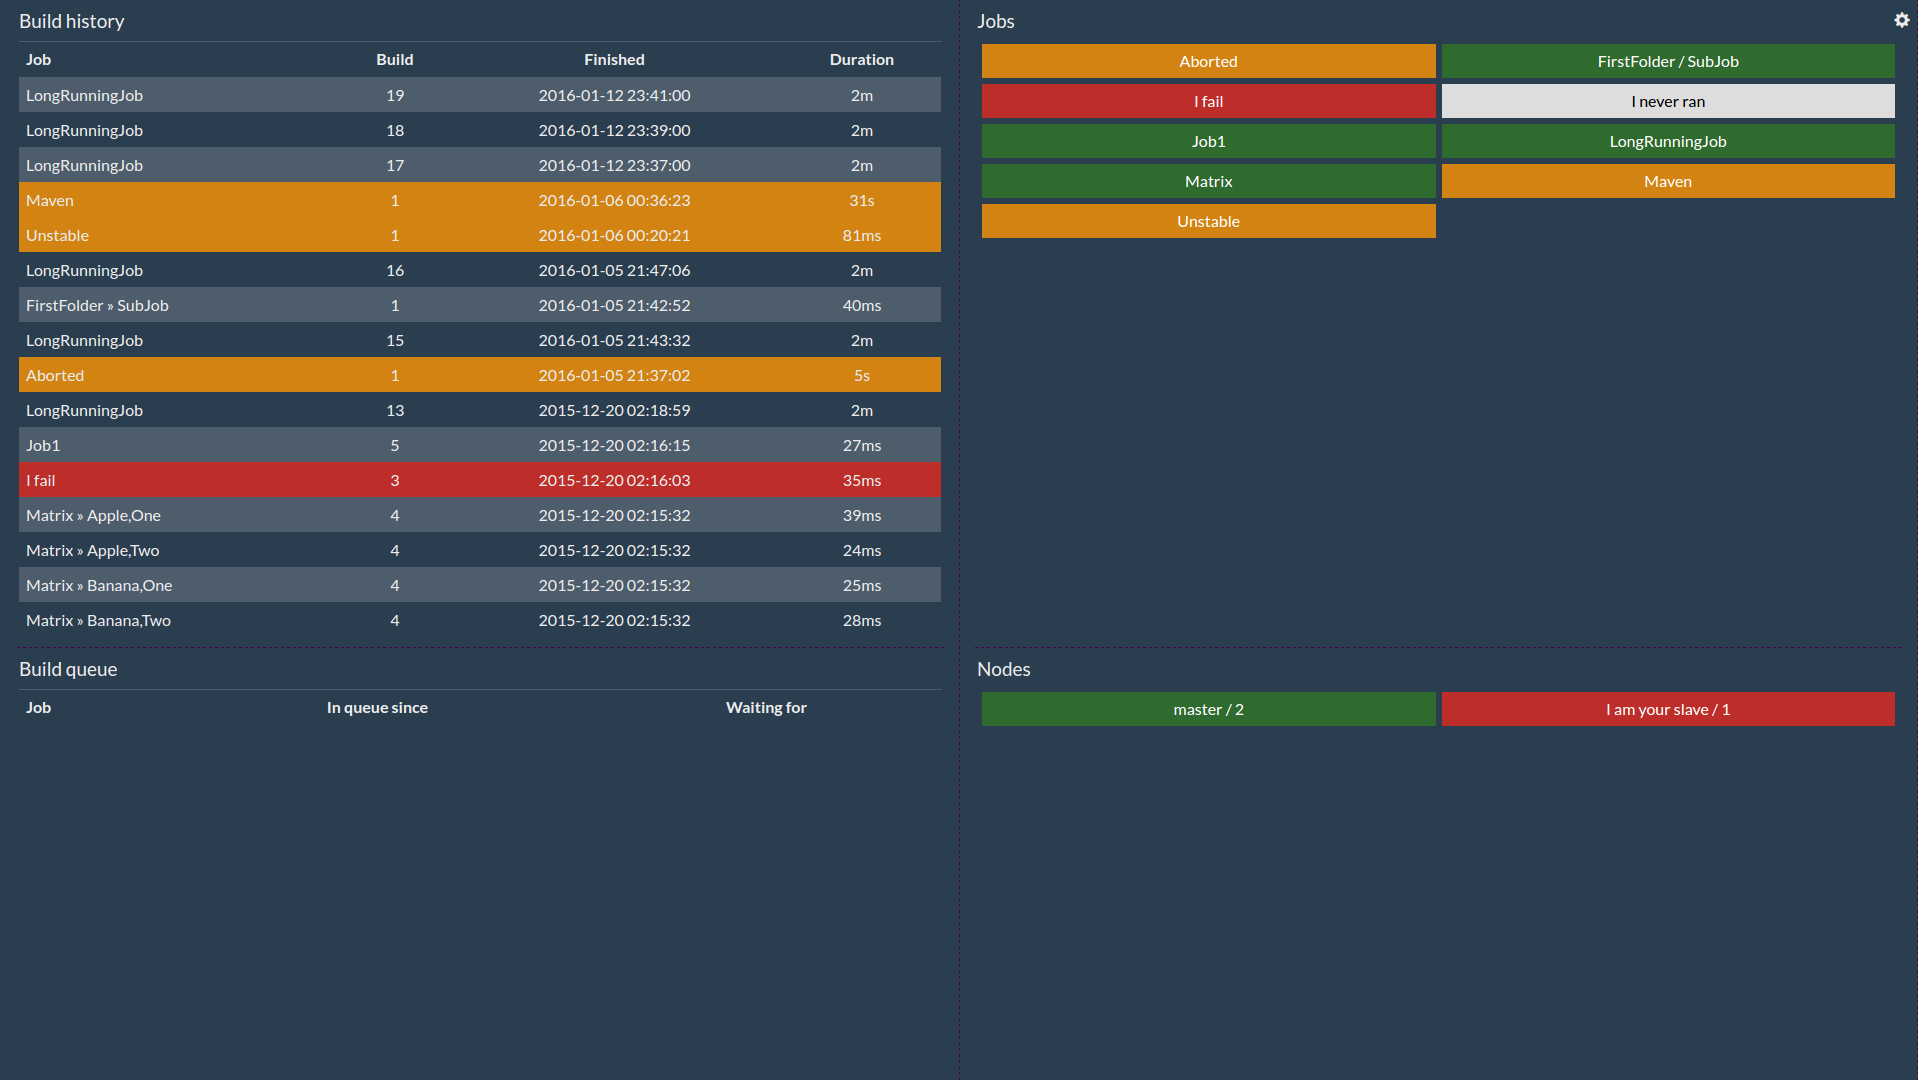
\includegraphics[width=1\textwidth]{missioncontrol}}
      \caption{Mission Control Plugin UI}
      \label{fig:missionControl}
  \end{figure}

\subsubsection{Metadata Plugin}\label{metadata_plugin}

Considering that one of the requirements is filtering the data displayed with the information of each test configuration, as said in section ~\ref{sec:res_system}, and since Jenkins has the possibility to store information on each of its CI items in XML format, exemplified in the figure~\ref{fig:buildXML}, then it could be stored some type of metadata as well.

To facilitate this, we used the extension point that Metadata Plugin~\cite{jkns:metadata} provides, in conjunction with the Jenkins API, to apply relevant filters on each job for an easier parsing of these configurations information.

  \begin{figure}[H]
  \centering
      \makebox[\textwidth][c]{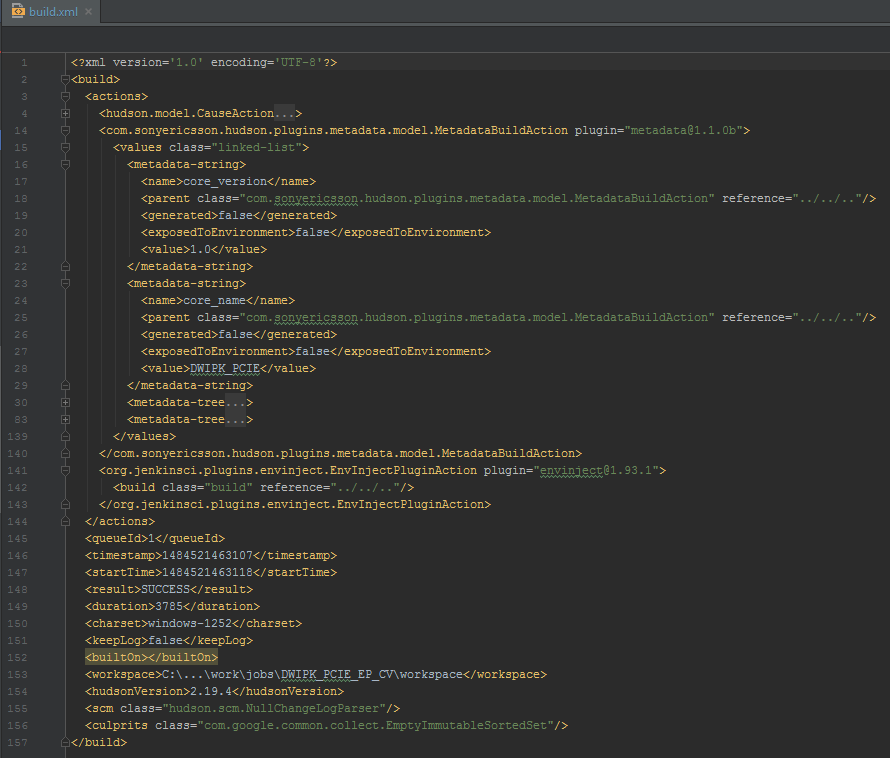
\includegraphics[width=1\textwidth]{buildXML}}
      \caption{XML file containing a Builds' information}
      \label{fig:buildXML}
  \end{figure}
  
This Metadata can be applied to Jobs simply through the customization menu, as seen in the figure~\ref{fig:metadataCustom}, which will apply it to every future Build after this point. 

  \begin{figure}[H]
  \centering
      \makebox[\textwidth][c]{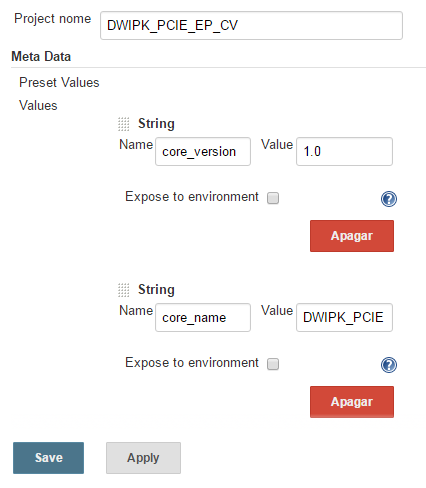
\includegraphics[width=0.5\textwidth]{metadataCustom}}
      \caption{Metadata option inside a Job customization panel}
      \label{fig:metadataCustom}
  \end{figure}

Or alternatively, automate the process simply by calling a post-build CLI command that is provided from the same plugin, using the format demonstrated in the figure~\ref{fig:updateMetadata}.

  \begin{figure}[H]
  \centering
      \makebox[\textwidth][c]{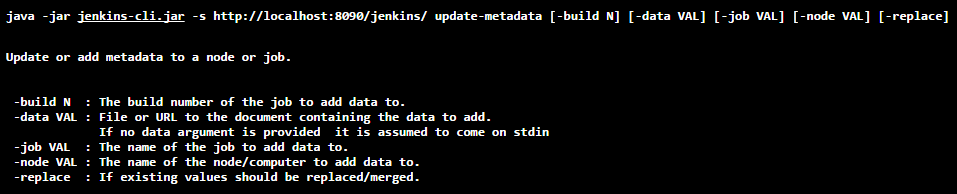
\includegraphics[width=1\textwidth]{updateMetadata}}
      \caption{CLI command update-metadata}
      \label{fig:updateMetadata}
  \end{figure}

\subsection{Server Side Implementation Design}\label{sc:implementationDesign}

Understanding how the back end in Java interacts with Jenkins and how projects were organized in Views, as explained in section \ref{sc:projOrg}, we defined a \textit{Top-down} strategy to obtain and parse the information of our items of interest.
This means we had to process View by View as individual projects to relate their child items in our Dashboard as seen in the figure~\ref{fig:dashboardDiagram}.

  \begin{figure}[H]
  \centering
      \makebox[\textwidth][c]{\includegraphics[width=1\textwidth]{dashboardDiagram}}
      \caption{\textit{Top-down} approach diagram}
      \label{fig:dashboardDiagram}
  \end{figure}
  
It was took in consideration the association between Views and Jobs inside Jenkins, namely that one Job is not associated to any View. Therefore each Job could be displayed multiple times, being represented by the same object.

We also needed a way to store information about the filters that can be applied, so we decided to implement a new Tag child in each Build. 

Based on this, our final plugin consists in this five different classes, depicted in the figure~\ref{fig:dash_uml}, that work together in parsing the information to display:

\begin{itemize}
\item \textbf{FilteredDashboardView - } The main class of the Dashboard. It collects all the Data from the Views selected and parses them into our other custom classes. After this collection, it exports the information to Jenkins API, which will be used to render and display in the front-end.

This class refreshes all the information when a new request is made by the front-end, which happens in a predefined time with an auto-refresh to capture new changes in the Jenkins instance, as schemed in the diagram \ref{fig:pluginInteraction}. 

We also ensure concurrency of the Views between all the life cycle of the class with a simple \code{CopyOnWriteArrayList<View> views = new CopyOnWriteArrayList<View>()} on its instantiation, which safeguards any View modification or deletion in the server. 

To ensure our approach scheme is followed, and prevent unnecessary duplicates of Jobs, these mapped in a variable \code{Map<String, JobData> jobsMap}, with their name serving as identifier, as well each Project mapped with its respective Jobs as \code{Map<String, ArrayList<String>> jobsInProjectMap}.

\item \textbf{Project - } Custom class representing a View. Contains a list of all Jobs inside the View as \code{ArrayList<JobData> projectJobs}. It is defined by its name \code{projectNane} and overall project status \code{projectStatus}. This status is calculated after all jobs are parsed and is set as the worst case scenario between them (i.e. if one Job fails, the whole project is set as \code{Fail}).

\item \textbf{JobData - } Custom class representing a Job. Contains a list of all Builds made by its represented Job as \code{ArrayList<Build> builds}. 

It has a subclass \textbf{JobVar} that keeps information of its variables, such as its URL, name and status. This concept was chosen for an easier access in the front-end, where we simply iterate through all these variables for display.

\item \textbf{Build -} Custom class representing a Build. Contains a list of Tags as  \code{ArrayList<Tag> tags} associated to this Build.

\item \textbf{Tag - } Class that represents a Metadata, from the plugin described in section ~\ref{metadata_plugin}, \code{label} and \code{value} contained in a Build, that will be used to apply filters in the Dashboard. Each \textbf{Tag} is the depiction of the configuration parameters utilized during the test process in section~\ref{sc:workflow}.
\end{itemize}

      \begin{figure}[H]
  \centering
      \makebox[\textwidth][c]{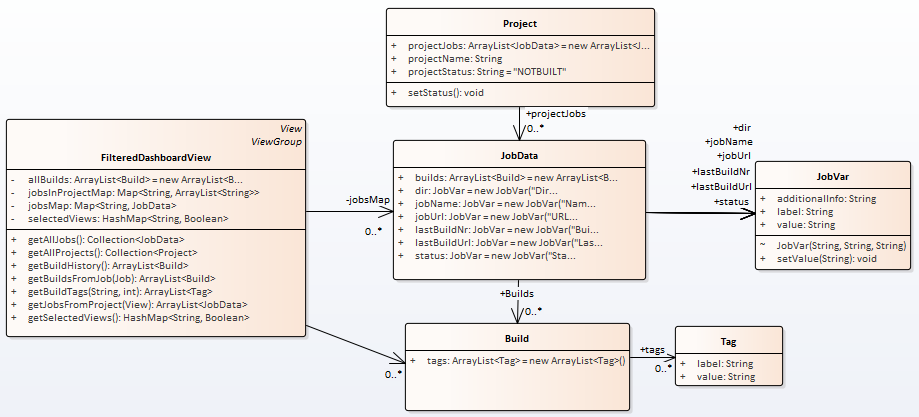
\includegraphics[width=1\textwidth]{dashboard_uml}}
      \caption{Filtered Dashboard View classes diagram}
      \label{fig:dash_uml}
  \end{figure}

      \begin{figure}[H]
  \centering
      \makebox[\textwidth][c]{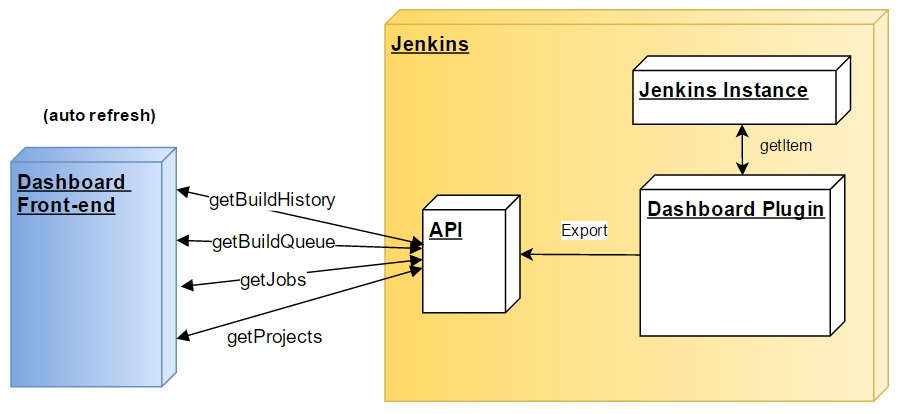
\includegraphics[width=1\textwidth]{frontBackConnection}}
      \caption{Interaction Diagram}
      \label{fig:pluginInteraction}
  \end{figure}

To eliminate some clustering of information, in the front-end we display only the last \textit{N} builds of each job. This number can be increased in the customization panel from figure \ref{fig:customize}, however it will also increase its processing time proportionally.

Finally, the addition of Tags to filter the information is the key feature of our Dashboard. This concept helps to maintain track of each configuration as requested in section \ref{sc:requirements}, with the minimum requisite of adding, or modifying, these labels to Jobs in the building process.

This design permits a totally scalable structure, since it has no limitations on the number of Views associated to the Dashboard, nor its Jobs and Builds. It can also be extendable to put more information in each of its custom classes for additional metrics and indicators in the future if desired. All this information only depends on the Jenkins API and what it supports.

\subsection{Front-End Implementation Design}\label{sc:frontend}

After the development of the server side, it was needed some brainstorming on how to organize the information structured and display it in the browser. 

For this, in the front-end display of the Dashboard, we based on the same scripts of the Mission Control Plugin, described in section~\ref{mission_plugin}, along with several common Web Application libraries and frameworks such as Javascript, jQuery and Bootstrap, all processed in Apache Jelly~\cite{jelly}, a Java and XML based scripting and processing engine that allows Jenkins its UI to be extended by plugins.

Since the data exported to the API is already well structured, the presentation process was completed with ease, only requiring a way to exhibit the view of a project with an intuitive display. 

To accomplish the aforementioned, was decided to display every Job inside the project as a column in a table, using the library referenced in section~\ref{sc:datatables}, being each row cell its Builds organized in a descending chronological order. Each cell has its Tags associated for a quick reference of the configurations utilized in the respective Build.



\subsubsection{Auxliary Library: DataTables - jQuery}\label{sc:datatables}

DataTables~\cite{dataTables} is a plugin for the jQuery Javascript library. 
It is a highly flexible tool that helped to create and add advanced interaction controls to any HTML table.

Is one of the key components of the front-end that made possible and simple the creation of a display table within the Dashboard, as well the search interaction with the added Tag filters.

\subsubsection{User Interface}\label{sc:ui}

Once the Dashboard is selected, it displays every View selected previously, as seen in the figure \ref{fig:createView}, and the overall status of those projects. It also shows all the Jobs inside those Views, and a Build history resulted from these, organized chronologically from the most recent. It is to note that every one of this items is linked directly to its object inside the Jenkins tool, eliminating the need of searching for them in the system.
  
In the figure~\ref{fig:mainDashb} its is shown the Synopsys IPK R\&D team's Dashboard, which are associated both HDMI and PCIe projects.
  
\begin{figure}[H]
  \centering
      \makebox[\textwidth][c]{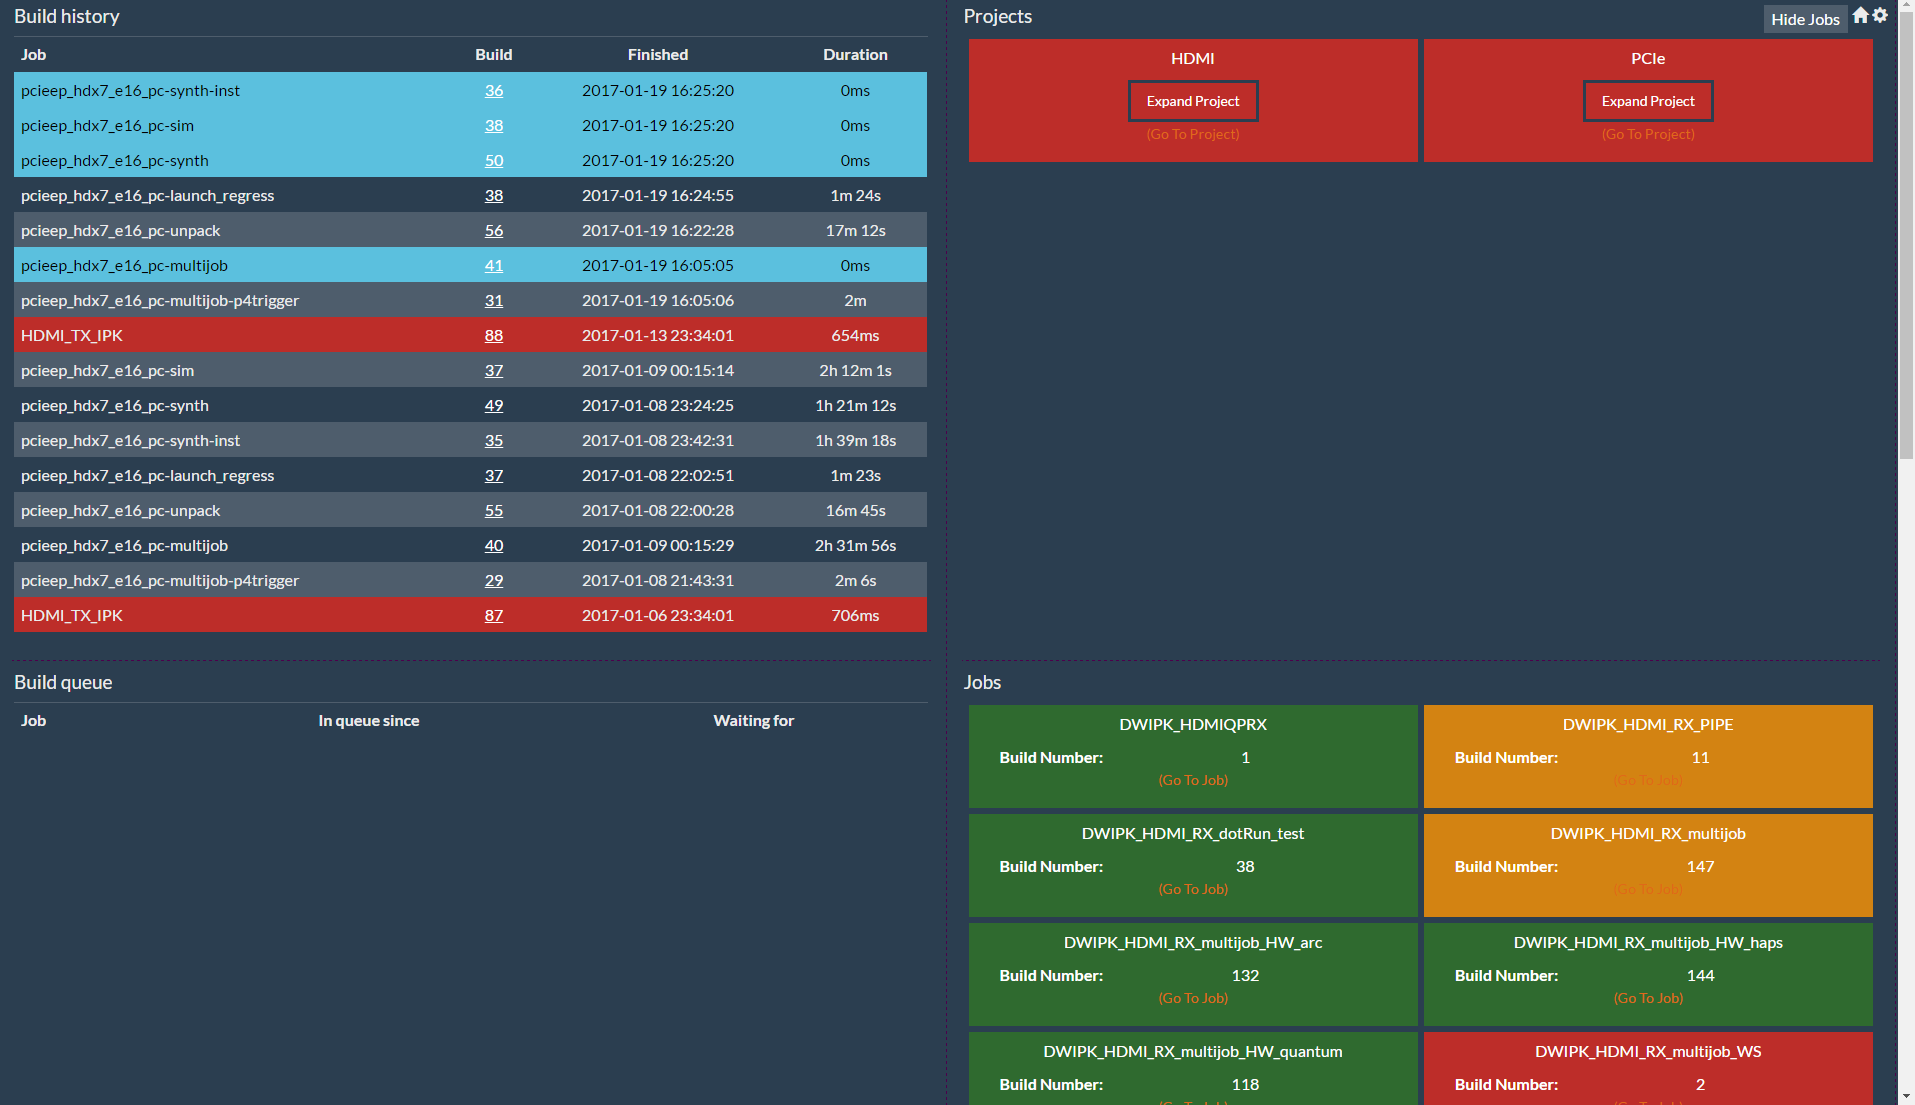
\includegraphics[width=1\textwidth]{maindashboard}}
      \caption{Dashboard Landing page}
      \label{fig:mainDashb}
  \end{figure}
  
It displays a "straight to the point" facet, that helps to identify exactly which Job or Build is not corresponding to the expected results.
 
  
Inside of each sub-view, the user can see information about Jobs, Builds and overall Project status, as well as the different filters defined by the Metadata inputs, referring to the different test configurations, displayed in the figure~\ref{dashboardTable1}. 
  
\begin{figure}[H]
  \centering
      \makebox[\textwidth][c]{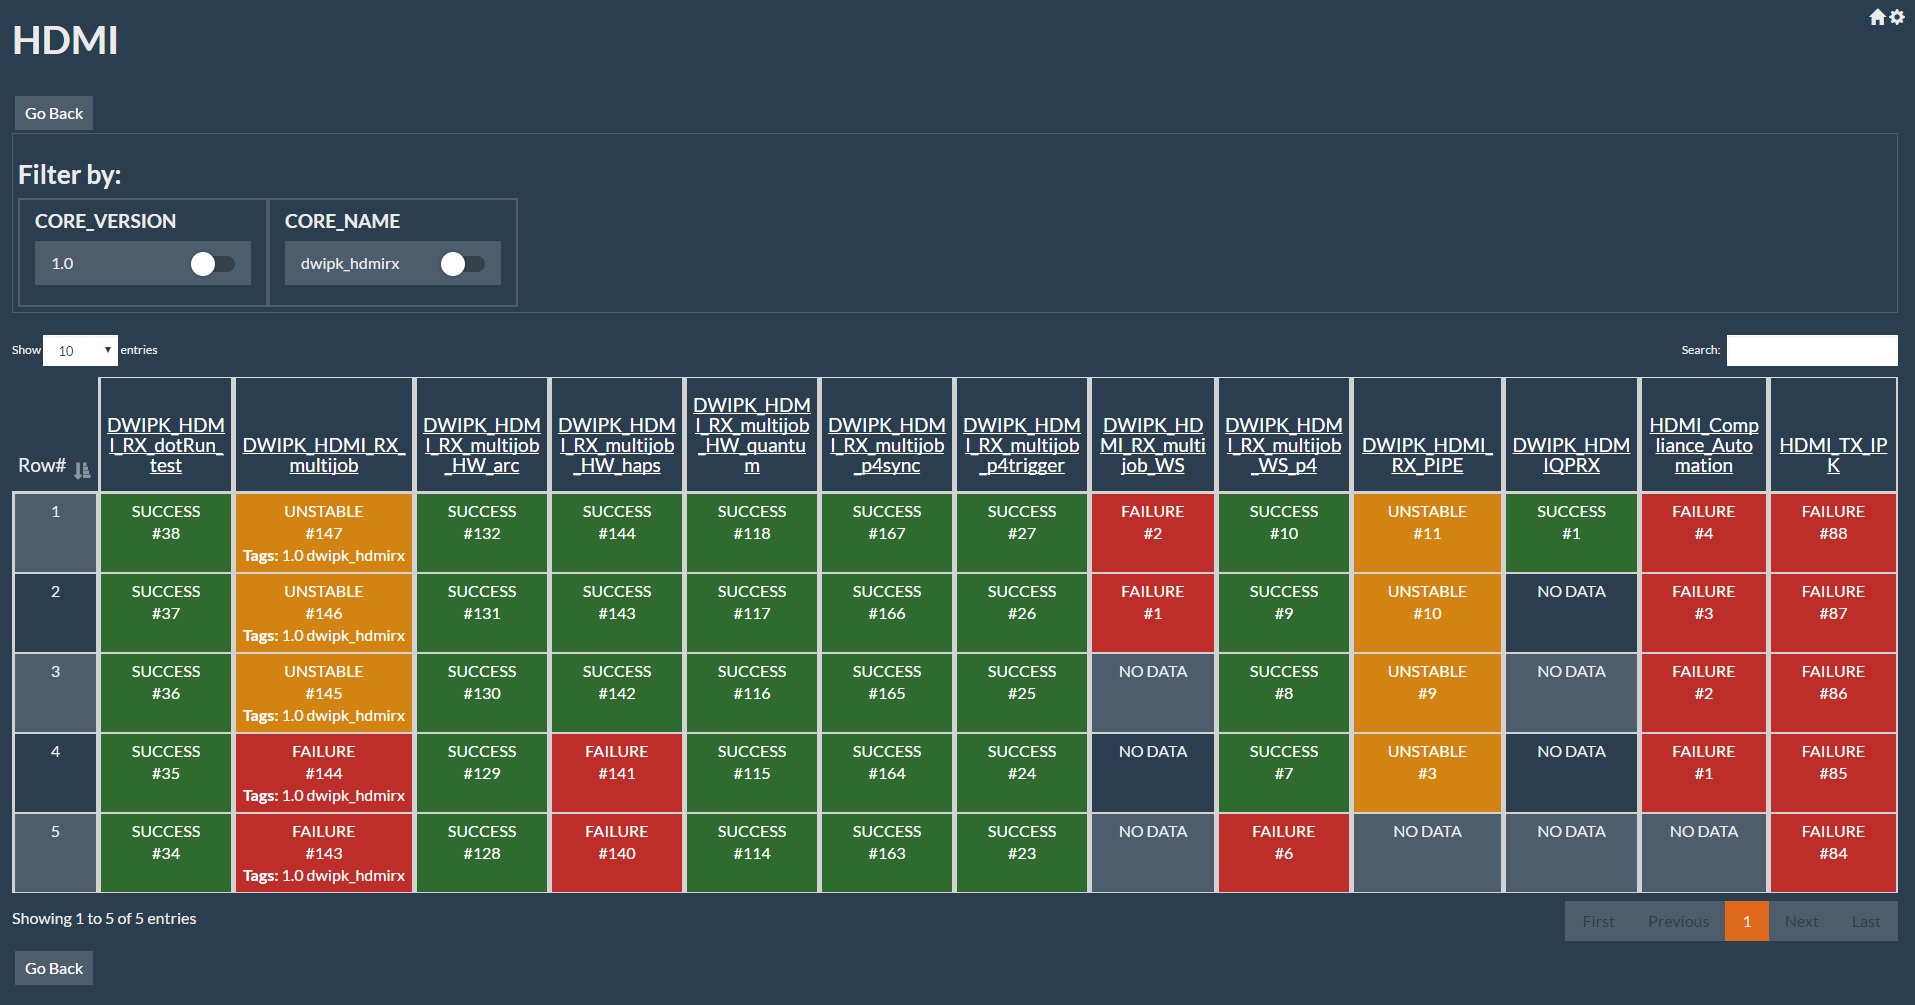
\includegraphics[width=1\textwidth]{dashboardtable1}}
      \caption{Overall view of a Project}
      \label{dashboardTable1}
  \end{figure}
  
For a quick filtering through the Tags, the user simply needs to select them in the respective section (Fig. \ref{dashboardTable2}). This search is made following a regular expression using the \code{AND} operator through all the selected Tags, displaying only the Builds that follow it. With this, we attain the desired streamlined perspective to troubleshoot and validate the configurations.
  
\begin{figure}[H]
  \centering
      \makebox[\textwidth][c]{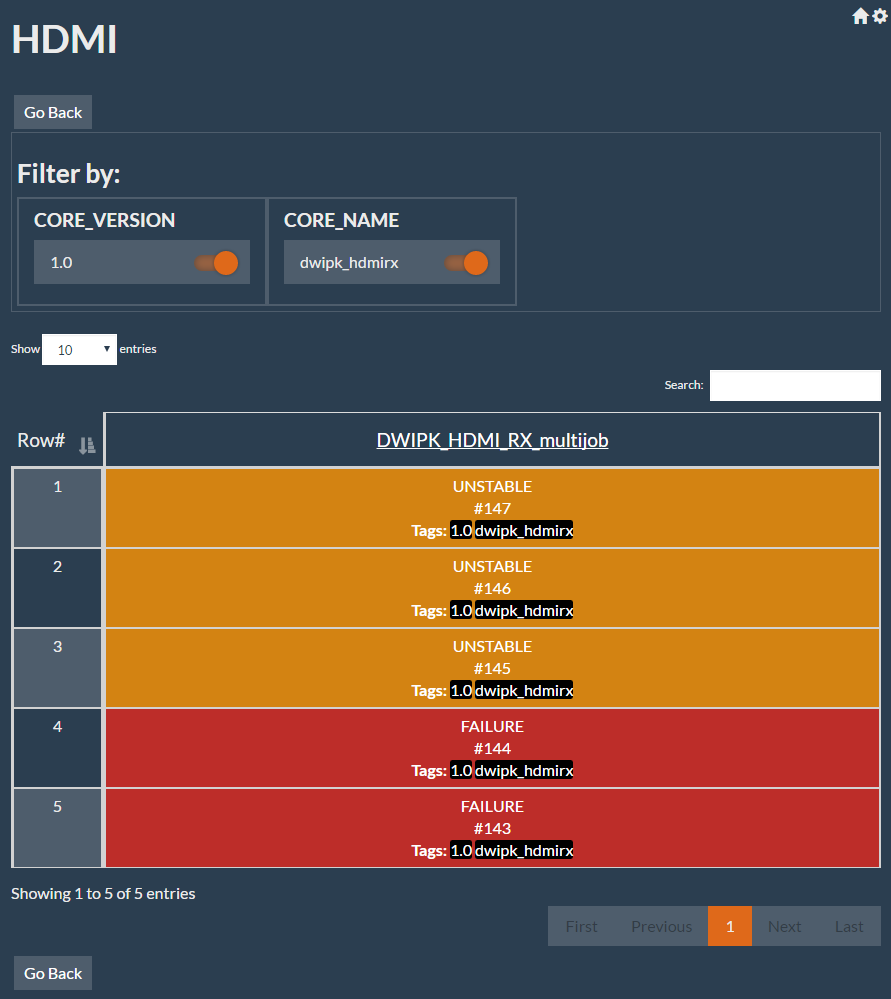
\includegraphics[width=0.6\textwidth]{dashboardtable2}}
      \caption{Overall view of the same Project (Fig.~\ref{dashboardTable1}) with filters applied}
      \label{dashboardTable2}
  \end{figure}

\section{Metadata and Pipeline Workaround}\label{workaraound}

One issue that was discovered while developing our plugin, was the incompatibility between the Metadata Plugin, from section \ref{metadata_plugin}, and the Pipeline Jobs~\cite{jnks:pipeline}. This occurs because the Metadata Plugin only supports Abstract Jobs, while Workflow Jobs (created in Pipeline) are not inherited from this class, since it was created in a pre-Workflow era.

To workaround this problem, it was created a function, exemplified in the snippet~\ref{groovy:setMetadata}, that can be patched in Pipeline Jobs groovy scripts and still maintain their complete functionality while being used in our Dashboard.

For this, one has to allow Pipeline builds to be Parameterized, as seen in figure \ref{fig:param}, and add String Parameters with the following structure: \(\textbf{metadata:}name\), where \(name\) can be any string the user wishes to reference the name of the metadata. This is valid because the inclusion of both Metadata and Parameters in Builds, are extended from the \code{Action} extension point of Jenkins.
Afterwards, only this function is needed in the Groovy script.

\begin{figure}[H]
  \centering
      \makebox[\textwidth][c]{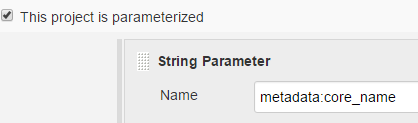
\includegraphics[width=0.6\textwidth]{parametrized}}
      \caption{Parameterized project selection}
      \label{fig:param}
  \end{figure}

\begin{lstlisting}[language=Java, label=groovy:setMetadata, caption=Groovy Script Workaround]
import hudson.model.*

@NonCPS
def setMetadata(map){
    def npl = new ArrayList<ParametersAction>();
    for(e in map){
        npl.add(new StringParameterValue(e.key.toString(), e.value.toString()));
    }
    def newPa = null
    def oldPa = currentBuild.build().getAction(ParametersAction.class)
    if (oldPa != null) {
        currentBuild.build().actions.remove(oldPa)
        newPa = oldPa.createUpdated(npl)
    } else {
        newPa = new ParametersAction(npl)
    }
    currentBuild.build().actions.add(newPa);
}
def map = [:]

//Example to populate the map:
map['metadata:core_name'] = 'DWIPK_HDMI_RX';
map['metadata:core_version'] = '1.0';
setMetadata(map);
\end{lstlisting}

This information will be parsed inside our dashboard with a condition statement, displayed in our snippet~\ref{java:pipelineIf} function, that creates exactly the same output for Pipelines as if other Job was being processed.

\begin{lstlisting}[language=Java, label=java:pipelineIf, caption=Java Condition Statement Workaround]
    public ArrayList<Tag> getBuildTags(String jobName, int buildNr) {
        ArrayList<Tag> tags = new ArrayList<Tag>();
        Job job = Jenkins.getInstance().getItemByFullName(jobName, Job.class);
        Run build = job.getBuildByNumber(buildNr);
        
        if (job.getClass().getName().equals("org.jenkinsci.plugins.workflow.job.WorkflowJob")) {
            ParametersAction parameterActions = build.getAction(ParametersAction.class);
            if (parameterActions != null) {
                for (ParameterValue parameter : parameterActions.getAllParameters()) {
                    if (parameter.getClass().equals(StringParameterValue.class)) {
                        if (StringUtils.substring(parameter.getName(), 0, "metadata:".length()).equals("metadata:") &&
                                !parameter.getValue().equals("")) {
                            String name = parameter.getName().replace("metadata:", "");
                            tags.add(new Tag(name.toUpperCase(), parameter.getValue().toString().toLowerCase()));
                        }
                    }
                }
            }
        }...        
      }      
\end{lstlisting}

\section{Conclusion}\label{sc:conclusion}

In this chapter the Dashboard solution was fully detailed along with the fixes one must do to make it fully functional with Pipelines. It is divided in simple classes that can be used as base for future extensions to the main View.

We can safely disclose that every obstacle in the previous Spreadsheet solution, detailed in section~\ref{sec:spreadsheet}, was surpassed:

\begin{itemize}
\item \textbf{Traceability - } The Dashboard is automatically updated when a new test is made.
\item \textbf{Susceptible to Human Error - } All the information comes from inside Jenkins, so there is no human interference in the process of displaying the information.
\item \textbf{Availability - } The only requirement is being a user inside the Jenkins tool and having permission to see the View.
\item \textbf{Difficulty to troubleshoot - } Every item on the Dashboard is linked directly to the original inside Jenkins, making the process a "one click" distance.
\end{itemize}

The plugin is made abstract enough so it can be used not only by our main target environment, but to help other software development teams equally. 

%%----------------------------------------
%% Final materials
%%----------------------------------------

%% Bibliography
%% Comment the next command if BibTeX file not used, 
%% Assumes that bibliography is in ``myrefs.bib''
\PrintBib{myrefs}

%% Comment next 2 commands if numbered appendices are not used
\appendix
\include{appendix1}

%% Index
%% Uncomment next command if index is required, 
%% don't forget to run ``makeindex pdis'' command
%\PrintIndex

\end{document}
